%********************************************************************
% Appendix
%*******************************************************
% If problems with the headers: get headings in appendix etc. right
\markboth{\spacedlowsmallcaps{Appendix}}{\spacedlowsmallcaps{Appendix}}
%************************************************
\chapter{Appendix: Preliminary Results on Other Gradient Estimators}\label{chap:appendix}

\section{Half-Cheetah Mujoco Task}
\vspace{-0.05in}
Here we present all the exploratory results for the versions introduced in section \ref{subsec:oge} for what concern the Half-Cheetah task. In this scenario we can't beat the baseline policy gradient algorithm in any case nor reach its performance. The performance confidence intervals of G(PO)MDP against \acs{SVRPG} are also disjoint for nearly all the learning process.
\begin{figure*}[h]
	\begin{minipage}[h]{1\textwidth}
		\centering
		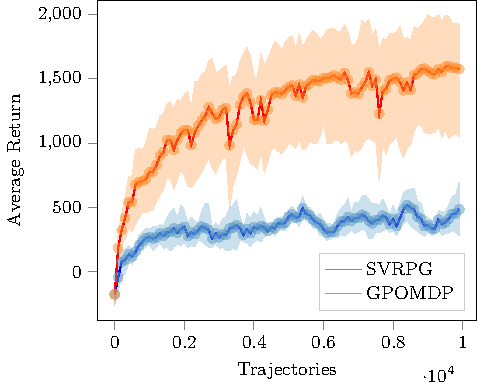
\includegraphics[width=0.75\textwidth]{Images/Experiments/half_cheetah_GPOMDP_vs_NonSelf_SVRPG_B.pdf}
		\vspace{-0.1in}
		\caption{On-line performance over sampled trajectories of \acs{SVRPG} B vs G(PO)MDP in the Half-Cheetah task, with 90\% bootstrap confidence intervals.}
		\label{fig:hcthree}
	\end{minipage}
	\vspace{-0.15in}
\end{figure*}
\begin{figure*}[h]
	\begin{minipage}[h]{1\textwidth}
		\centering
		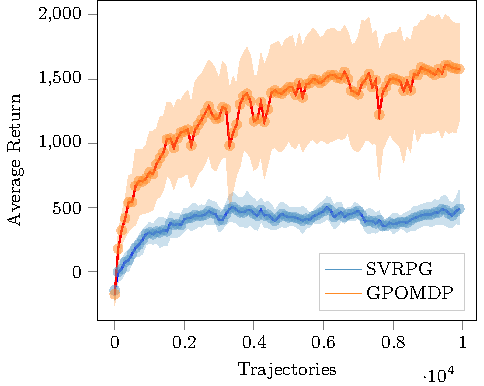
\includegraphics[width=0.75\textwidth]{Images/Experiments/half_cheetah_GPOMDP_vs_NonSelf_SVRPG_C.pdf}
		\vspace{-0.1in}
		\caption{On-line performance over sampled trajectories of \acs{SVRPG} C vs G(PO)MDP in the Half-Cheetah task, with 90\% bootstrap confidence intervals.}
		\label{fig:hcfour}
	\end{minipage}
	\vspace{-0.15in}
\end{figure*}

\begin{figure*}[h]
	\begin{minipage}[h]{1\textwidth}
		\centering
		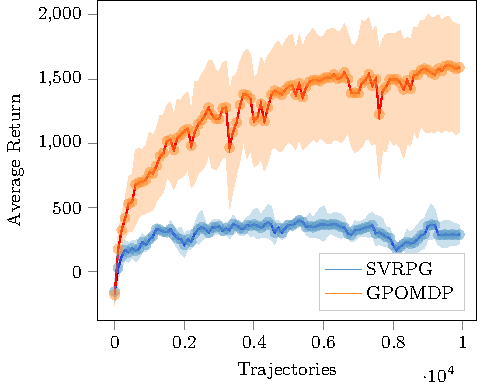
\includegraphics[width=0.75\textwidth]{Images/Experiments/half_cheetah_GPOMDP_vs_SVRPG_B_reuse.pdf}
		\vspace{-0.1in}
		\caption{On-line performance over sampled trajectories of \acs{SVRPG} BR vs G(PO)MDP in the Half-Cheetah task, with 90\% bootstrap confidence intervals.}
		\label{fig:hcnine}
	\end{minipage}
	\vspace{-0.15in}
\end{figure*}

\begin{figure*}[h]
	\begin{minipage}[h]{1\textwidth}
		\centering
		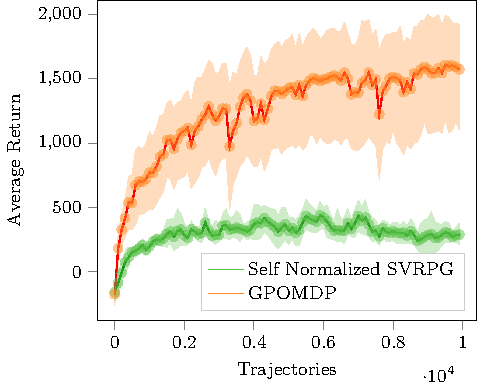
\includegraphics[width=0.75\textwidth]{Images/Experiments/half_cheetah_GPOMDP_vs_SN_SVRPG_B.pdf}
		\vspace{-0.1in}
		\caption{On-line performance over sampled trajectories of Self Normalized \acs{SVRPG} B vs G(PO)MDP in the Half-Cheetah task, with 90\% bootstrap confidence intervals.}
		\label{fig:hcfive}
	\end{minipage}
	\vspace{-0.15in}
\end{figure*}
\begin{figure*}[h]
	\begin{minipage}[h]{1\textwidth}
		\centering
		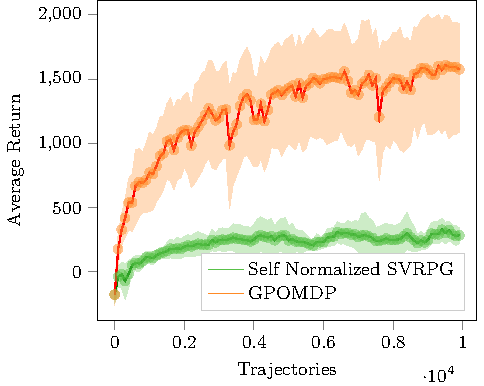
\includegraphics[width=0.75\textwidth]{Images/Experiments/half_cheetah_GPOMDP_vs_SN_SVRPG_C.pdf}
		\vspace{-0.1in}
		\caption{On-line performance over sampled trajectories of Self Normalized \acs{SVRPG} C vs G(PO)MDP in the Half-Cheetah task, with 90\% bootstrap confidence intervals.}
		\label{fig:hcsix}
	\end{minipage}
	\vspace{-0.15in}
\end{figure*}

\begin{figure*}[h]
	\begin{minipage}[h]{1\textwidth}
		\centering
		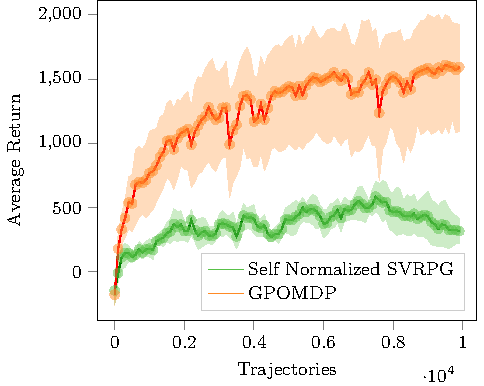
\includegraphics[width=0.75\textwidth]{Images/Experiments/half_cheetah_GPOMDP_vs_SN_SVRPG_B_reuse.pdf}
		\vspace{-0.1in}
		\caption{On-line performance over sampled trajectories of Self Normalized \acs{SVRPG} BR vs G(PO)MDP in the Half-Cheetah task, with 90\% bootstrap confidence intervals.}
		\label{fig:hcten}
	\end{minipage}
	\vspace{-0.15in}
\end{figure*}


\begin{figure*}[h]
	\begin{minipage}[h]{1\textwidth}
		\centering
		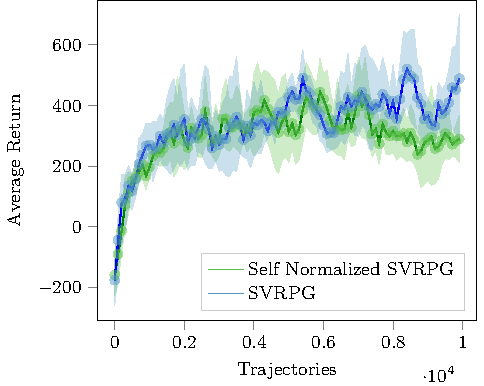
\includegraphics[width=0.75\textwidth]{Images/Experiments/half_cheetah_SVRPG_vs_SN_SVRPG_B.pdf}
		\vspace{-0.1in}
		\caption{On-line performance over sampled trajectories of Self Normalized \acs{SVRPG} B vs \acs{SVRPG} B in the Half-Cheetah task, with 90\% bootstrap confidence intervals.}
		\label{fig:hcseven}
	\end{minipage}
	\vspace{-0.15in}
\end{figure*}
\begin{figure*}[h]
	\begin{minipage}[h]{1\textwidth}
		\centering
		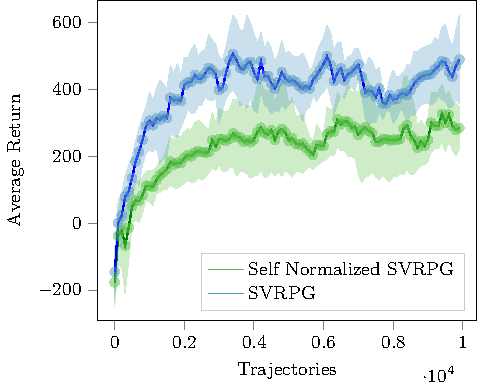
\includegraphics[width=0.75\textwidth]{Images/Experiments/half_cheetah_SVRPG_vs_SN_SVRPG_C.pdf}
		\vspace{-0.1in}
		\caption{On-line performance over sampled trajectories of Self Normalized \acs{SVRPG} C vs \acs{SVRPG} C in the Half-Cheetah task, with 90\% bootstrap confidence intervals.}
		\label{fig:hcheight}
	\end{minipage}
	\vspace{-0.15in}
\end{figure*}

\begin{figure*}[h]
	\begin{minipage}[h]{1\textwidth}
		\centering
		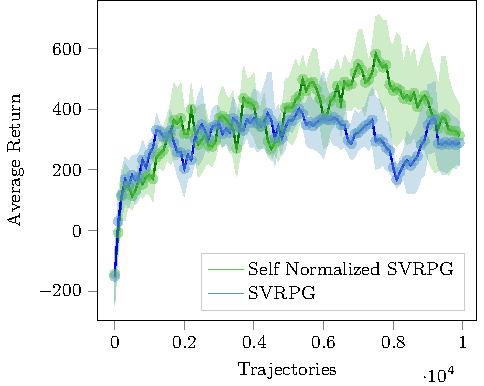
\includegraphics[width=0.75\textwidth]{Images/Experiments/half_cheetah_SVRPG_vs_SN_SVRPG_B_reuse.pdf}
		\vspace{-0.1in}
		\caption{On-line performance over sampled trajectories of Self Normalized \acs{SVRPG} BR vs \acs{SVRPG} BR in the Half-Cheetah task, with 90\% bootstrap confidence intervals.}
		\label{fig:hceleven}
	\end{minipage}
	\vspace{-0.15in}
\end{figure*}

\clearpage
\section{Swimmer Mujoco Task}
\vspace{-0.05in}
Here we present all the exploratory results for the versions introduced in section \ref{subsec:oge} for what concert the Swimmer task. As previously said, this task is simpler than half-cheetah (see the previous section), indeed, we have better results \wrt version B and BR. More precisely, if we have a look to figure \ref{fig:swimmerfive} we can see how the B version of \acs{SVRPG} without self-normalization is able, near the end of the learning process, to reach the performace of the baseline G(PO)MPD. Whereas, in figure \ref{fig:swimmersix} we see how \acs{SVRPG} BR is able, for a small fraction of the learning process, to outperform G(PO)MDP at least in terms of expected performance (the result, as you can see from the confidence interval, is not statistically significant). Unfortunately we still experience the ineffectiveness of \acs{SVRPG} C which, as we can see in figure \ref{fig:swimmerfour}, is not able to reach the baseline performance. If we try to use self normalization we experience a shrinkage over the performance \wrt the related non self normalized algorithm (see figures \ref{fig:swimmerthree}, \ref{fig:swimmerseven} and \ref{fig:swimmereight}).

\begin{figure*}[h]
	\begin{minipage}[h]{1\textwidth}
		\centering
		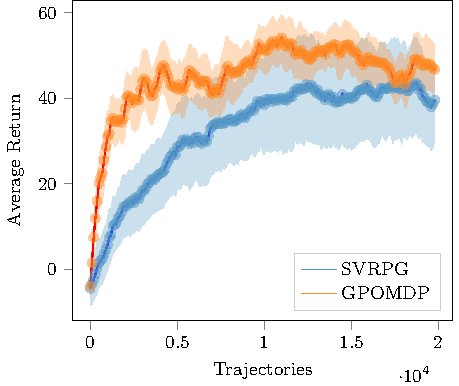
\includegraphics[width=0.75\textwidth]{Images/Experiments/swimmer_SVRPG_vs_GPOMDP_B.pdf}
		\vspace{-0.1in}
		\caption{On-line performance over sampled trajectories of \acs{SVRPG} B vs G(PO)MDP in the Swimmer task, with 90\% bootstrap confidence intervals.}
		\label{fig:swimmerfive}
	\end{minipage}
	\vspace{-0.15in}
\end{figure*}

\begin{figure*}[h]
	\begin{minipage}[h]{1\textwidth}
		\centering
		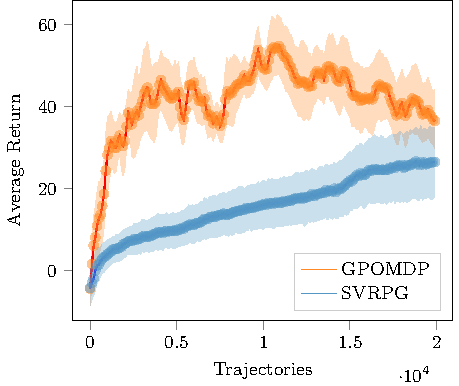
\includegraphics[width=0.75\textwidth]{Images/Experiments/swimmer_SVRPG_vs_GPOMDP_C.pdf}
		\vspace{-0.1in}
		\caption{On-line performance over sampled trajectories of \acs{SVRPG} C vs G(PO)MDP in the Swimmer task, with 90\% bootstrap confidence intervals.}
		\label{fig:swimmerfour}
	\end{minipage}
	\vspace{-0.15in}
\end{figure*}

\begin{figure*}[h]
	\begin{minipage}[h]{1\textwidth}
		\centering
		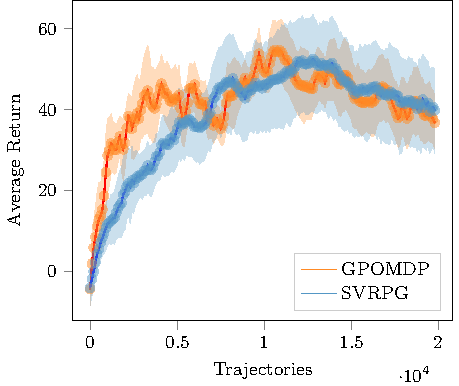
\includegraphics[width=0.75\textwidth]{Images/Experiments/swimmer_GPOMDP_vs_SVRPG_B_reuse.pdf}
		\vspace{-0.1in}
		\caption{On-line performance over sampled trajectories of \acs{SVRPG} BR vs G(PO)MDP in the Swimmer task, with 90\% bootstrap confidence intervals.}
		\label{fig:swimmersix}
	\end{minipage}
	\vspace{-0.15in}
\end{figure*}


\begin{figure*}[h]
	\begin{minipage}[h]{1\textwidth}
		\centering
		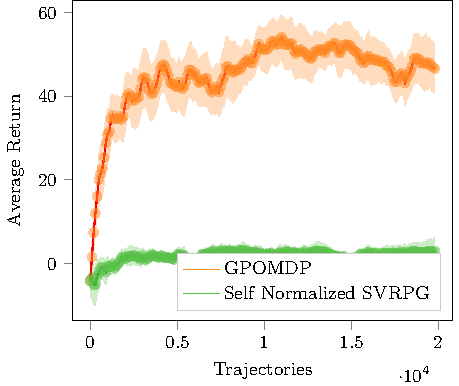
\includegraphics[width=0.75\textwidth]{Images/Experiments/swimmer_Self_SVRPG_vs_GPOMDP_B.pdf}
		\vspace{-0.1in}
		\caption{On-line performance over sampled trajectories of Self Normalized \acs{SVRPG} B vs G(PO)MDP in the Swimmer task, with 90\% bootstrap confidence intervals.}
		\label{fig:swimmerthree}
	\end{minipage}
	\vspace{-0.15in}
\end{figure*}

\begin{figure*}[h]
	\begin{minipage}[h]{1\textwidth}
		\centering
		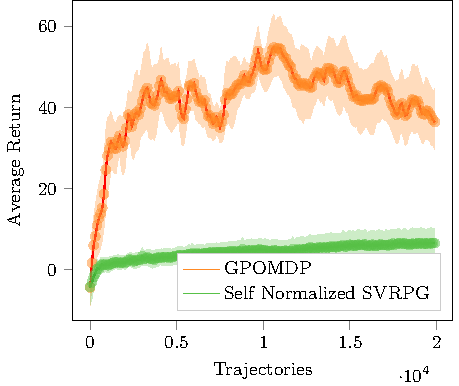
\includegraphics[width=0.75\textwidth]{Images/Experiments/swimmer_GPOMDP_vs_SN_SVRPG_C.pdf}
		\vspace{-0.1in}
		\caption{On-line performance over sampled trajectories of \acs{SVRPG} C vs G(PO)MDP in the Swimmer task, with 90\% bootstrap confidence intervals.}
		\label{fig:swimmerseven}
	\end{minipage}
	\vspace{-0.15in}
\end{figure*}

\begin{figure*}[h]
	\begin{minipage}[h]{1\textwidth}
		\centering
		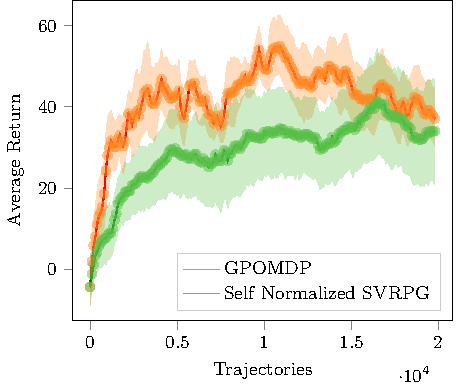
\includegraphics[width=0.75\textwidth]{Images/Experiments/swimmer_GPOMDP_vs_SN_SVRPG_B_reuse.pdf}
		\vspace{-0.1in}
		\caption{On-line performance over sampled trajectories of \acs{SVRPG} BR vs G(PO)MDP in the Swimmer task, with 90\% bootstrap confidence intervals.}
		\label{fig:swimmereight}
	\end{minipage}
	\vspace{-0.15in}
\end{figure*}


\begin{figure*}[h]
	\begin{minipage}[h]{1\textwidth}
		\centering
		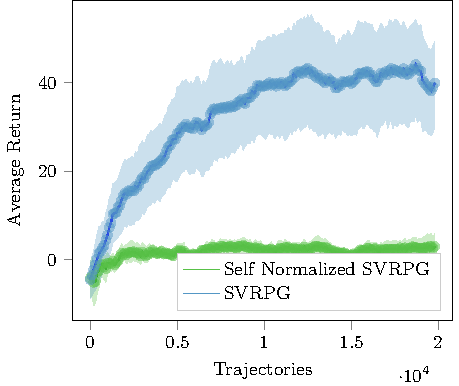
\includegraphics[width=0.75\textwidth]{Images/Experiments/swimmer_SVRPG_vs_sn_SVRPG_B.pdf}
		\vspace{-0.1in}
		\caption{On-line performance over sampled trajectories of Self Normalized \acs{SVRPG} B vs \acs{SVRPG} B in the Swimmer task, with 90\% bootstrap confidence intervals.}
		\label{fig:swimmernine}
	\end{minipage}
	\vspace{-0.15in}
\end{figure*}
\begin{figure*}[h]
	\begin{minipage}[h]{1\textwidth}
		\centering
		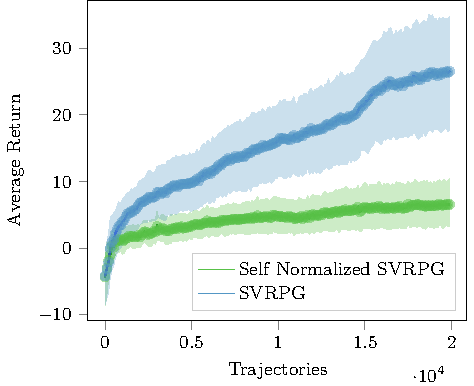
\includegraphics[width=0.75\textwidth]{Images/Experiments/swimmer_SVRPG_vs_sn_SVRPG_C.pdf}
		\vspace{-0.1in}
		\caption{On-line performance over sampled trajectories of Self Normalized \acs{SVRPG} C vs \acs{SVRPG} C in the Swimmer task, with 90\% bootstrap confidence intervals.}
		\label{fig:swimmerten}
	\end{minipage}
	\vspace{-0.15in}
\end{figure*}

\begin{figure*}[h]
	\begin{minipage}[h]{1\textwidth}
		\centering
		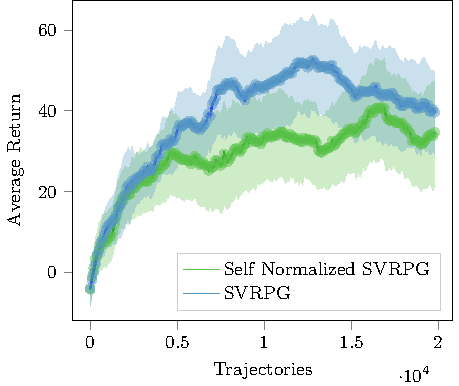
\includegraphics[width=0.75\textwidth]{Images/Experiments/swimmer_SVRPG_vs_SN_SVRPG_B_reuse.pdf}
		\vspace{-0.1in}
		\caption{On-line performance over sampled trajectories of Self Normalized \acs{SVRPG} BR vs \acs{SVRPG} BR in the Swimmer task, with 90\% bootstrap confidence intervals.}
		\label{fig:swimmereleven}
	\end{minipage}
	\vspace{-0.15in}
\end{figure*}



\clearpage
\vspace{-0.05in}
\section{Cart-Pole Task}
\vspace{-0.05in}
Here we present all the exploratory results for the versions introduced in section \ref{subsec:oge} for what concert the Cart-Pole task. This is the simplest task we tackled in this composition, indeed, the versions which in the previous sections were nearly as good as the baseline G(PO)MDP now works perfectly. As we can see figure \ref{fig:cartpole1} shows \acs{SVRPG} B outperforming G(PO)MDP and the same holds for \acs{SVRPG} BR in figure \ref{fig:cartpole2}. Note that the BR version is better than our principal algorithm with this task. For what concern the \acs{SVRPG} C we still have inconclusive results as shown in figure \ref{fig:cartpole3}.

\begin{figure*}[h]
	\begin{minipage}[h]{1\textwidth}
		\centering
		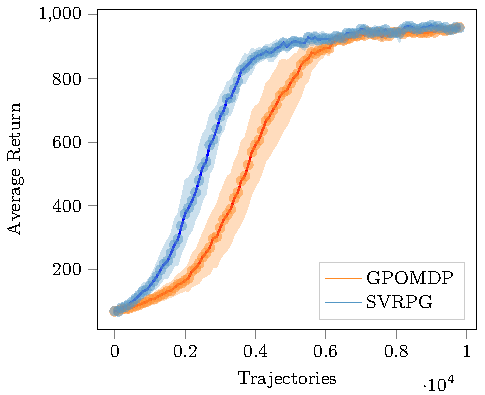
\includegraphics[width=0.75\textwidth]{Images/Experiments/cart_pole_GPOMDP_vs_SVRPG_B.pdf}
		\vspace{-0.1in}
		\caption{On-line performance over sampled trajectories of \acs{SVRPG} B vs G(PO)MDP in the Cart-Pole task, with 90\% bootstrap confidence intervals.}
		\label{fig:cartpole1}
	\end{minipage}
	\vspace{-0.15in}
\end{figure*}


\begin{figure*}[h]
	\begin{minipage}[h]{1\textwidth}
		\centering
		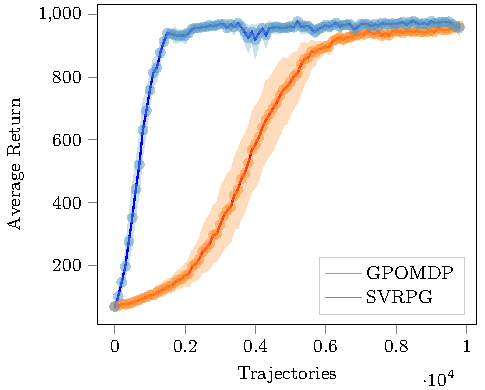
\includegraphics[width=0.75\textwidth]{Images/Experiments/cart_pole_GPOMDP_vs_SVRPG_B_reuse.pdf}
		\vspace{-0.1in}
		\caption{On-line performance over sampled trajectories of \acs{SVRPG} BR vs G(PO)MDP in the Cart-Pole task, with 90\% bootstrap confidence intervals.}
		\label{fig:cartpole2}
	\end{minipage}
	\vspace{-0.15in}
\end{figure*}
\clearpage
\begin{figure*}[h]
	\begin{minipage}[h]{1\textwidth}
		\centering
		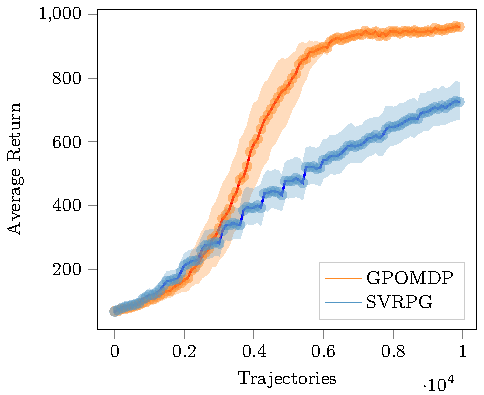
\includegraphics[width=0.75\textwidth]{Images/Experiments/cart_pole_GPOMDP_vs_SVRPG_C.pdf}
		\vspace{-0.1in}
		\caption{On-line performance over sampled trajectories of \acs{SVRPG} C vs G(PO)MDP in the Cart-Pole task, with 90\% bootstrap confidence intervals.}
		\label{fig:cartpole3}
	\end{minipage}
	\vspace{-0.15in}
\end{figure*}
